\chapter{Simulazioni e Risultati}
\section{Set-up Numerico}
In questo capitolo si discutono le simulazioni effettuate e si analizzano i risultati con l'obiettivo di trovare il miglior modello, sia rispetto agli episodi di allenamento, sia rispetto agli altri modelli che presentano parametri diversi. Per affrontare in maniera consistente questo processo, si definiscono nella tab.\ref{tab:model_params} i parametri che caratterizzano nell'interezza un modello DDPG e nella tab.\ref{tab:model_metrics} le metriche utilizzate nel giudizio di questi ultimi.
\newline

Nella fig.\ref{fig:tracks} si vede a sinistra il tracciato utilizzato per il training dei modelli e a destra quello utilizzato per la validazione.

\begin{figure}[hb]
    \centering
    
\includegraphics[width = 3.5in]{Figures/Chapter5/training_test_track.png}
    \caption{Tracciati di training e validazione}
    \label{fig:tracks}
\end{figure}

\clearpage


\begin{table}[hb]
\centering
\begin{tabular}{|cl|}
\hline
\multicolumn{1}{|c|}{\textbf{Nome}}  & \multicolumn{1}{c|}{\textbf{Descrizione}}                                                                                    \\ \hline
\multicolumn{1}{|c|}{MEM\_SIZE}      & Dimensione dell'experience replay                                                                                            \\ \hline
\multicolumn{1}{|c|}{BATCH\_SIZE}    & \begin{tabular}[c]{@{}l@{}}Dimensione del batch di transizioni prelevate\\ contemporaneamente dall'experience replay\end{tabular} \\ \hline
\multicolumn{1}{|c|}{DC\_FACT}       & Discount Factor $\gamma$ del Q Learning                                                                         \\ \hline
\multicolumn{1}{|c|}{SM\_FACT}       & Fattore di smooth $\tau$ utilizzato nel soft update                                                             \\ \hline
\multicolumn{1}{|c|}{CLR}            & Learning rate del Critic e del Target Critic                                                                                 \\ \hline
\multicolumn{1}{|c|}{ALR}            & Learning rate dell'Actor e del Target Actor                                                                                  \\ \hline
\multicolumn{1}{|c|}{C\_1} & \begin{tabular}[c]{@{}l@{}}Numero di neuroni del primo livello denso\\ nascosto del Critic e del Target Critic\end{tabular}  \\ \hline
\multicolumn{1}{|c|}{C\_2} & \begin{tabular}[c]{@{}l@{}}Numero di neuroni del secondo livello denso\\ nascosto del Critic e del Target Critic\end{tabular}     \\ \hline
\multicolumn{1}{|c|}{A\_1}  & \begin{tabular}[c]{@{}l@{}}Numero di neuroni del primo livello denso\\ nascosto dell'Actor e del Target Actor\end{tabular}   \\ \hline
\multicolumn{1}{|c|}{A\_2}  & \begin{tabular}[c]{@{}l@{}}Numero di neuroni del secondo livello denso\\ nascosto dell'Actor e del Target Actor\end{tabular} \\ \hline
\multicolumn{1}{|c|}{NOISE}          & Rumore esplorativo scelto per il modello                                                                                     \\ \hline
\multicolumn{1}{|c|}{REWARD}         & Reward scelta per il modello                                                                                      \\ \hline
\end{tabular}
\caption{Parametri del modello}
\label{tab:model_params}
\end{table}

\begin{table}[hb]
\centering
\begin{tabular}{|cl|}
\hline
\multicolumn{1}{|c|}{\textbf{Nome}}   & \multicolumn{1}{c|}{\textbf{Descrizione}} \\ \hline
\multicolumn{1}{|c|}{EPISODIC\_REWARD} & Reward cumulativa di un episodio          \\ \hline
\multicolumn{1}{|c|}{MSE\_TRACKPOS} &
  \begin{tabular}[c]{@{}l@{}}Mean Squared Error della trackPos rispetto al centro \\ della carreggiata (ovvero trackPos = 0) di un episodio\end{tabular} \\ \hline
\multicolumn{1}{|c|}{N\_STEPS}         & Numero di step che compongono l'episodio (max 6000)     \\ \hline
\end{tabular}
\caption{Metriche di giudizio}
\label{tab:model_metrics}
\end{table}




\clearpage

\subsection{Panoramica dei modelli allenati}

Nella tab.\ref{tab:tests} sono presentati tutti i modelli che sono stati allenati insieme ai valori dei loro parametri.
\newline

Non tutti i parametri hanno subito variazioni durante i test, pertanto nella tab.\ref{tab:predef_value} sono presentati tali parametri e i loro valori predefiniti.

\begin{table}[hb]
\centering
\begin{tabular}{|c|c|}
\hline
\multicolumn{1}{|l|}{\textbf{Parametro}} & \multicolumn{1}{l|}{\textbf{Valore}} \\ \hline
MEM\_SIZE                                 & 100000                               \\ \hline
BATCH\_SIZE                               & 64                                   \\ \hline
DC\_FACT                                  & 0,99                                 \\ \hline
SM\_FACT                                  & 0,001                                \\ \hline
CLR                                      & 0,001                                \\ \hline
ALR                                      & 0,0001                               \\ \hline
C\_1                                      & 300                               \\ \hline
C\_2                                      & 400                               \\ \hline
A\_1                                      & 300                               \\ \hline
A\_2                                      & 400                               \\ \hline
\end{tabular}
\caption{Valore predefinito dei parametri immutati}
\label{tab:predef_value}
\end{table}

\begin{table}[hb]
\centering
\begin{tabular}{|c|c|c|c|c|c|c|}
\hline
\multicolumn{1}{|l|}{\textbf{MODEL\_ID}} &
  \multicolumn{1}{l|}{\textbf{NOISE}} &
  \multicolumn{1}{l|}{\textbf{REWARD}} \\ \hline
1 & OU      & standard    \\ \hline
2 & TVNoise & standard    \\ \hline
3 & GN      & standard    \\ \hline
4 & OU      & no trackPos \\ \hline
5 & OU      & angle       \\ \hline
\end{tabular}
\caption{Modelli e rispettivi parametri}
\label{tab:tests}
\end{table}

\clearpage



\section{Scelta del modello DDPG}

Lo scopo di questa sezione è evidenziare il miglior modello tra quelli presentati, rispetto ai parametri che hanno subito variazioni. 

\subsection{Modalità del confronto tra modelli}\label{confronto_modelli}

Ogni confronto ha lo scopo di evidenziare il miglior episodio di allenamento di un modello, rispetto alla variazione di un parametro, sia tra tutti i modelli sotto test che tra gli episodi di allenamento del modello stesso.
\newline

Per la valutazione si procede come segue:
\begin{enumerate}
    \item Si prelevano i 100 episodi di allenamento di ogni modello che hanno il maggior N\_STEPS.
    \item Di questi, si selezionano solamente i 30 episodi che hanno il minor MSE\_TRACKPOS.
    \item Di questi, si seleziona l'episodio di ciascun modello che ha la EPISODIC\_REWARD più grande.
    \item Infine si seleziona l'episodio del modello che, tra tutti quelli sotto test, ha la maggior EPISODIC\_REWARD.
\end{enumerate}

\clearpage

\subsection{Test sul tipo di rumore}

In questo test si mettono a paragone i tre tipi di rumore utilizzati: l'OU Modificato, il GN e il TVNoise. Si testeranno, quindi, il Modello 1, 2 e 3.
\newline

In fig.\ref{fig:model_1}, \ref{fig:model_2}, \ref{fig:model_3} vengono mostrati gli andamenti delle metriche di interesse rispetto agli episodi di testing dei tre modelli. Da sinistra verso destra, rispettivamente, EPISODIC\_REWARD, N\_STEPS, MSE\_TRACKPOS.


Alla fine dei primi 3 passi della valutazione rimane da confrontare l'episodio 415 del Modello 1 con quello 493 del Modello 2 e quello 451 del Modello 3. Come si vede in tab.\ref{tab:models_1-2-3}, il Modello 1 presenta una EPISODIC\_REWARD maggiore dei Modelli 2 e 3.
\newline
Gli MSE\_TRACKPOS dei Modelli 1 e 2 sono comparabili mentre il Modello 3 ha performance di tracking notevolmente inferiori ai primi due.
\newline

In questo caso, nel rispetto delle modalità di confronto definite, il Modello 1 risulta il migliore.

\begin{table}[hb]
\centering
\resizebox{\textwidth}{!}{%
\begin{tabular}{|c|c|c|c|c|}
\hline
\multicolumn{1}{|l|}{{\color[HTML]{000000} \textbf{MODEL\_ID}}} &
  {\color[HTML]{000000} \textbf{EPISODIO}} &
  {\color[HTML]{000000} \textbf{EPISODIC\_REWARD}} &
  \multicolumn{1}{l|}{\textbf{MSE\_TRACKPOS}} &
  \multicolumn{1}{l|}{\textbf{N\_STEPS}} \\ \hline
{\color[HTML]{000000} 1} &
  {\color[HTML]{000000} 415} &
  {\color[HTML]{000000} 510353} &
  0,022 &
  6000 \\ \hline
{\color[HTML]{000000} 2} &
  {\color[HTML]{000000} 493} &
  {\color[HTML]{000000} 483797} &
  0,015 &
  6000 \\ \hline
{\color[HTML]{000000} 3} &
  {\color[HTML]{000000} 451} &
  {\color[HTML]{000000} 400165} &
  0,088 &
  6000 \\ \hline
\end{tabular}%
}
\caption{Confronto Modelli 1, 2 e 3}
\label{tab:models_1-2-3}
\end{table}

\begin{figure}[hb]
    \centering
    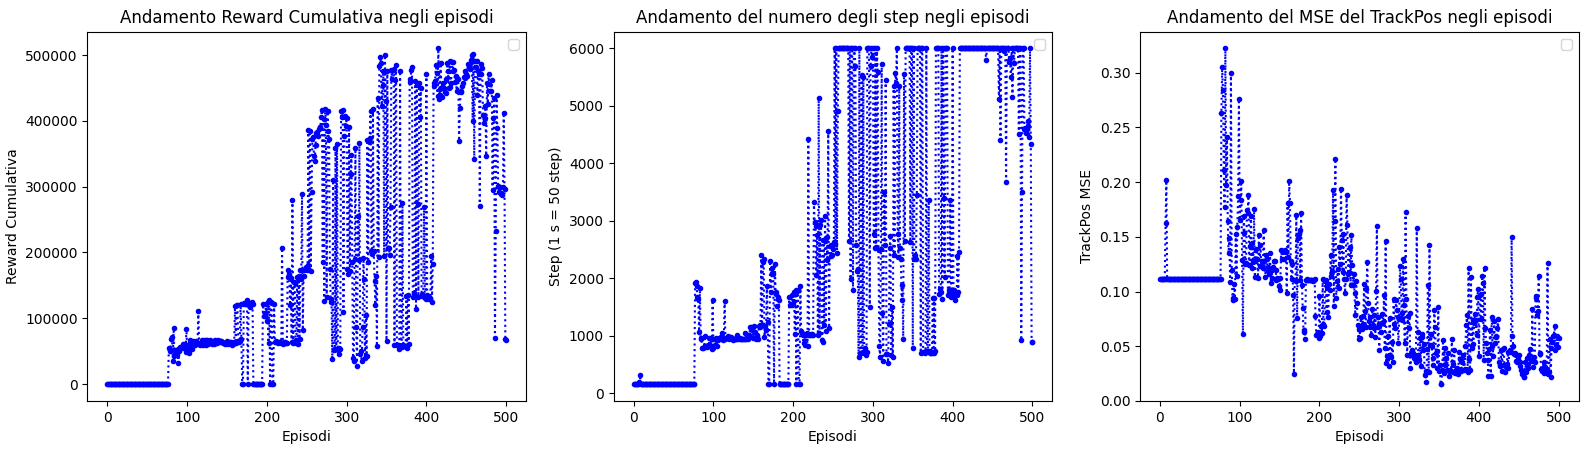
\includegraphics[width = 6in]{Figures/Chapter5/model_1.png}
    \caption{Statistiche del Modello 1}
    \label{fig:model_1}
\end{figure}

\begin{figure}[hb]
    \centering
    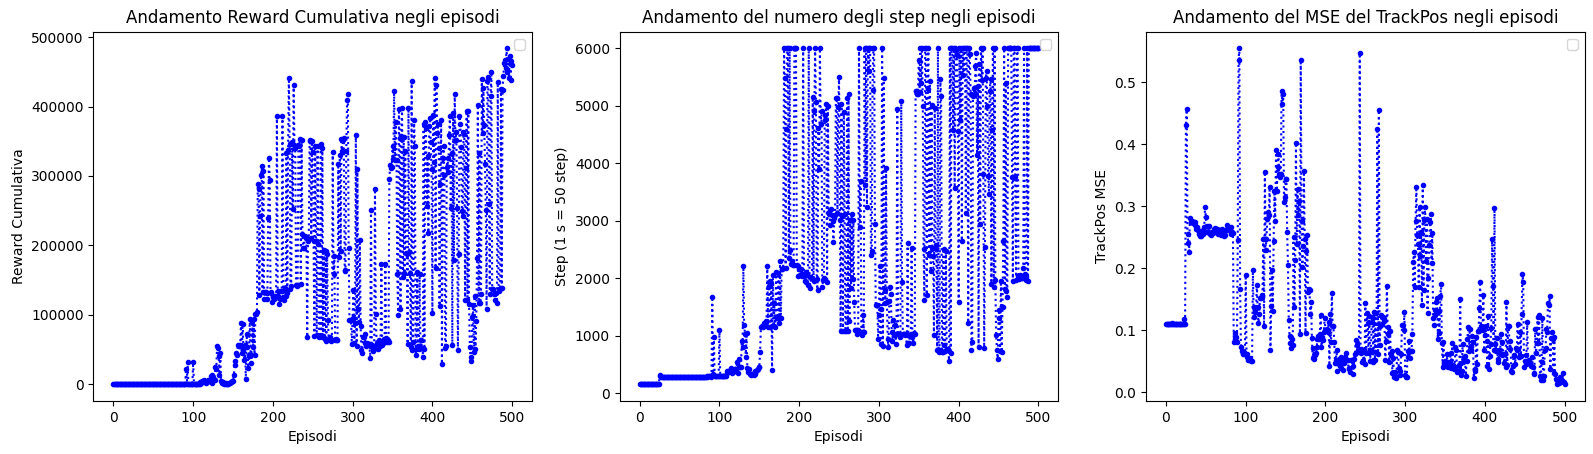
\includegraphics[width = 6in]{Figures/Chapter5/model_2.png}
    \caption{Statistiche del Modello 2}
    \label{fig:model_2}
\end{figure}

\begin{figure}[hb]
    \centering
    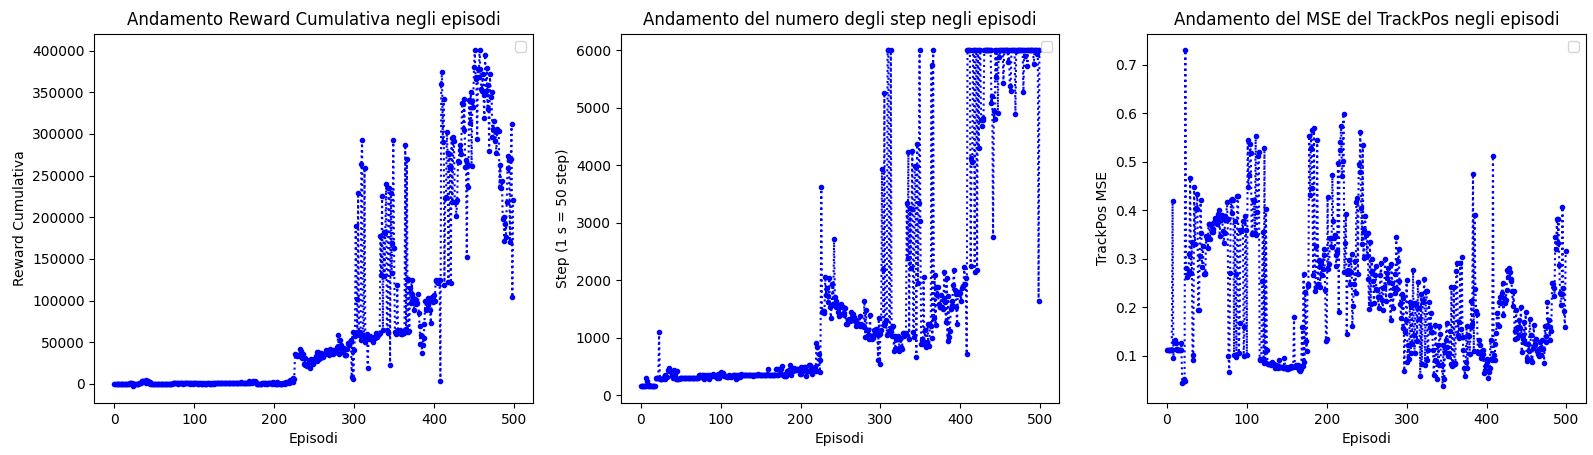
\includegraphics[width = 6in]{Figures/Chapter5/model_3.png}
    \caption{Statistiche del Modello 3}
    \label{fig:model_3}
\end{figure}

\clearpage

\subsection{Test sul tipo di reward function}

Per verificare quale reward function porti risultati migliori, si mettono a paragone i Modelli 1, 4 e 5. Nella fig.\ref{fig:model_4} si mostrano gli andamenti delle metriche del Modello 4, mentre nella fig.\ref{fig:model_5} quelli del Modello 5.

\begin{figure}[hb]
    \centering
    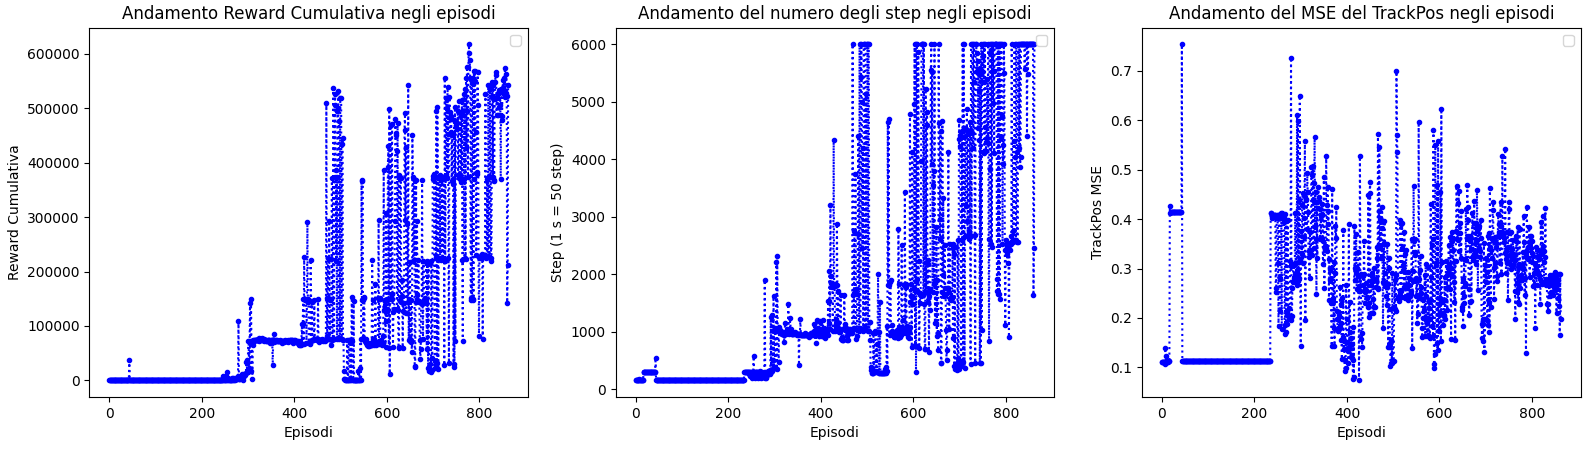
\includegraphics[width = 6in]{Figures/Chapter5/model_4.png}
    \caption{Statistiche del Modello 4}
    \label{fig:model_4}
\end{figure}

\begin{figure}[hb]
    \centering
    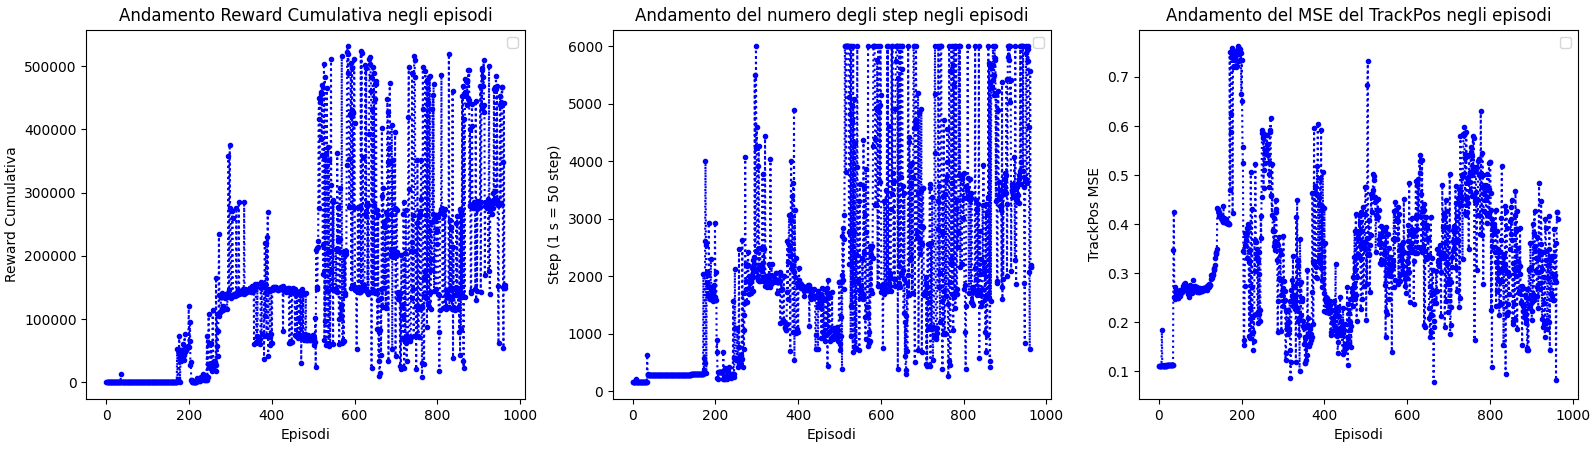
\includegraphics[width = 6in]{Figures/Chapter5/model_5.png}
    \caption{Statistiche del Modello 5}
    \label{fig:model_5}
\end{figure}

Alla fine dei primi 3 passi della valutazione rimangono da confrontare l'episodio 415 del Modello 1, l'episodio 778 del Modello 4 e l'episodio 583 del Modello 5.

\clearpage

Come si nota dalla tab.\ref{tab:models_1-4-5}, i Modelli 4 e 5 hanno una EPISODIC\_REWARD maggiore di quella del Modello 1. Tuttavia si riconosce che il Modello 1 riesce a mantenere un MSE\_TRACKPOS dieci volte più basso rispetto a quello degli altri due modelli.
\newline

Riassumendo, quindi, l'utilizzo di una reward che include il controllo puntuale della trackPos, come quella definita in \ref{rewardfunction}, favorisce l'allenamento di un modello che segue pedissequamente il centro della carreggiata, mentre l'utilizzo di una reward come quelle definite in \ref{rewardfunction_notrackpos} e \ref{rewardfunction_angle} porta all'allenamento di un agente che, seppur mantenendosi sempre entro i limiti della carreggiata, riesce ad elaborare strategie di guida più audaci che portano a ricompense più alte perché è in grado di sfruttatare meglio la conformazione della pista.
\newline

In ultima analisi si osserva che il Modello 5, il quale implementa una reward con controllo sull'angolo del veicolo, ha un MSE\_TRACKPOS maggiore di quello del Modello 4. Questo ci fa concludere che la reward più funzionale alla risoluzione del problema proposto è quella del Modello 4.

\begin{table}[hb]
\centering
\resizebox{\textwidth}{!}{%
\begin{tabular}{|c|c|c|c|c|}
\hline
\multicolumn{1}{|l|}{{\color[HTML]{000000} \textbf{MODEL\_ID}}} &
  {\color[HTML]{000000} \textbf{EPISODIO}} &
  {\color[HTML]{000000} \textbf{EPISODIC\_REWARD}} &
  \multicolumn{1}{l|}{\textbf{MSE\_TRACKPOS}} &
  \multicolumn{1}{l|}{\textbf{N\_STEPS}} \\ \hline
{\color[HTML]{000000} 1} &
  {\color[HTML]{000000} 415} &
  {\color[HTML]{000000} 510353} &
  0,022 &
  6000 \\ \hline
{\color[HTML]{000000} 4} & {\color[HTML]{000000} 778} & {\color[HTML]{000000} 601018} & 0,276 & 6000 \\ \hline
5                        & 583                        & 531486                        & 0,284 & 6000 \\ \hline
\end{tabular}%
}
\caption{Confronto Modelli 1, 4 e 5}
\label{tab:models_1-4-5}
\end{table}

\subsection{Modello finale}

Il Modello 4 e il Modello 5 risultano essere, nel complesso, i due miglior modelli secondo le modalità di confronto definite. Il Modello 4, però, riesce ad ottenere performance molto più alte in termini di EPISODIC\_REWARD, quindi è scelto come modello definitivo nell'episodio 778.
\newline

\clearpage

\section{Risultati numerici}

In questa sezione vengono presentati i risultati numerici ottenuti sul tracciato di validazione dal Modello 4 nell'episodio 778 e confrontati con quelli del Modello 1 nell'episodio 415.
\newline

Nella fig.\ref{fig:model_1-4_reward}, \ref{fig:model_1-4_velocity} e \ref{fig:model_1-4_trackpos} vengono mostrati, rispettivamente, l'andamento della reward, l'andamento della velocità e l'andamento dell'errore quadratico della trackPos dei due modelli nei due rispettivi episodi migliori. Nell'analisi della \ref{fig:model_1-4_trackpos} si tenga presente che il Modello 4 implementa una reward che non impone il mantenimento del centro della carreggiata bensì solo di rimanere all'interno di quest'ultima. Per tale ragione si considera buono ogni risultato minore di 1.

\begin{figure}[hb]
    \centering
    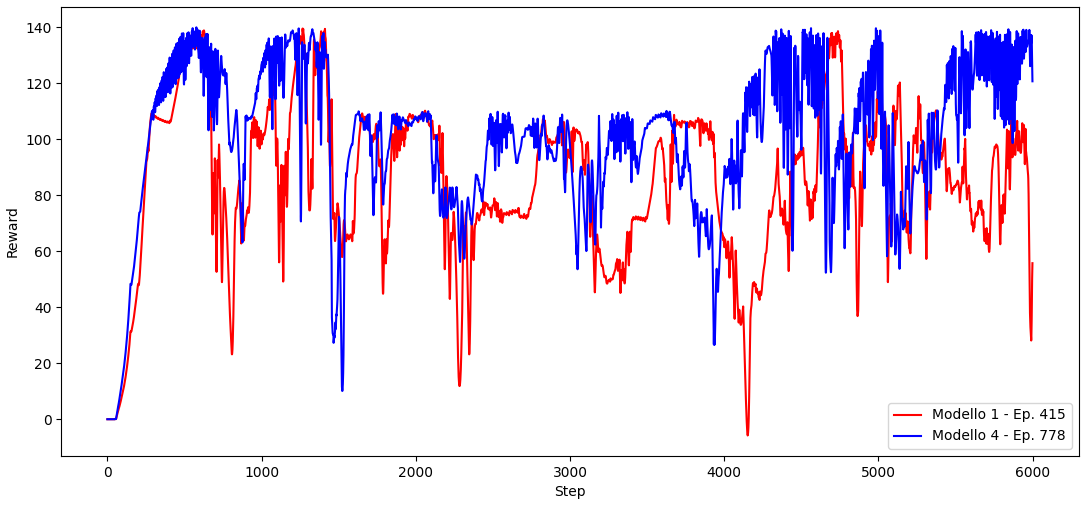
\includegraphics[width = 5.5in]{Figures/Chapter5/model_1-4_reward.png}
    \caption{Reward nell'episodio}
    \label{fig:model_1-4_reward}
\end{figure}

\begin{figure}[hb]
    \centering
    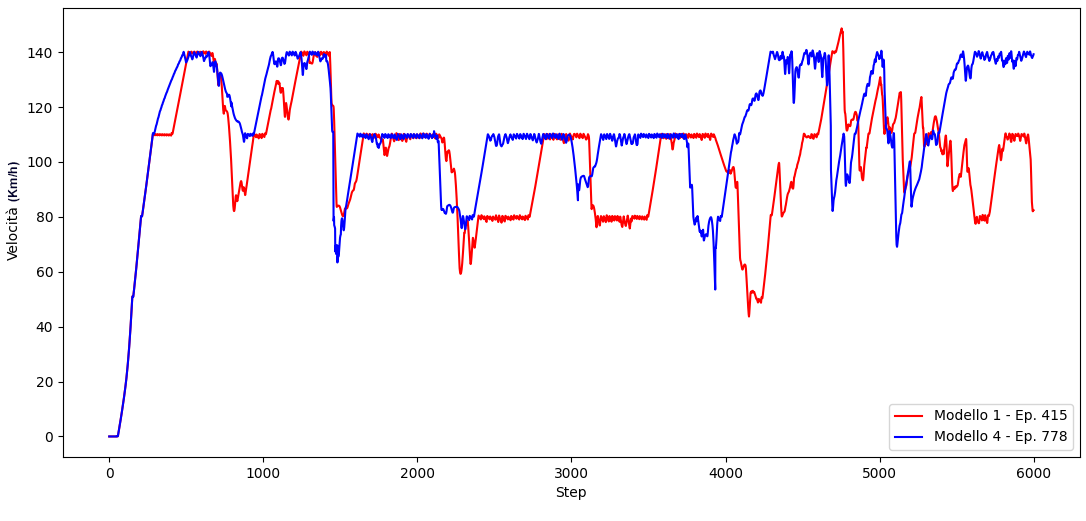
\includegraphics[width = 5.5in]{Figures/Chapter5/model_1-4_velocity.png}
    \caption{Velocità nell'episodio}
    \label{fig:model_1-4_velocity}
\end{figure}

\begin{figure}[hb]
    \centering
    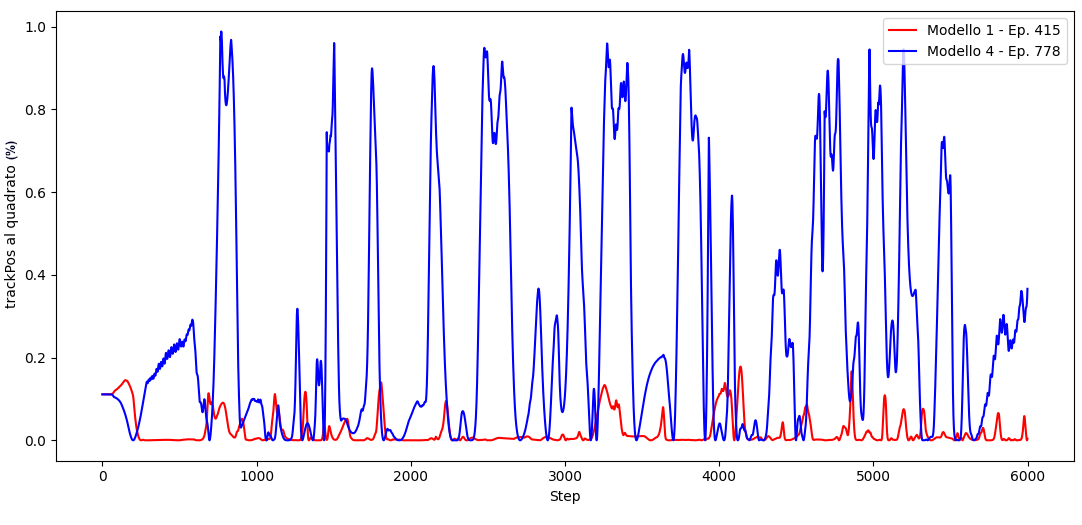
\includegraphics[width = 5.5in]{Figures/Chapter5/model_1-4_trackpos.png}
    \caption{Errore quadratico trackPos nell'episodio}
    \label{fig:model_1-4_trackpos}
\end{figure}